\documentclass[10pt]{article}

\usepackage{geometry}
\geometry{a4paper, margin=0.7in, top=0.55in, bottom=0.55in}

\usepackage{titling}
\usepackage{graphicx}
\usepackage{hyperref}
\usepackage{booktabs}
\usepackage{array}
\usepackage{makecell}
\usepackage{enumitem}
\usepackage{subcaption}
\usepackage{float}
\usepackage{listings}
\usepackage{xcolor}
\usepackage{amsmath}
\usepackage{amssymb}
\usepackage{amsfonts}
\usepackage[justification=centering]{caption}

\definecolor{codegreen}{rgb}{0,0.6,0}
\definecolor{codegray}{rgb}{0.5,0.5,0.5}
\definecolor{codepurple}{rgb}{0.58,0,0.82}
\definecolor{backcolour}{rgb}{0.97,0.97,0.97}

\lstset{
	language=Python,
	backgroundcolor=\color{backcolour},
	commentstyle=\color{codegreen}\itshape,
	keywordstyle=\color{blue}\bfseries,
	numberstyle=\tiny\color{codegray},
	stringstyle=\color{codepurple},
	basicstyle=\ttfamily\scriptsize,
	breakatwhitespace=false,
	breaklines=true,
	captionpos=b,
	keepspaces=true,
	numbers=left,
	numbersep=5pt,
	showspaces=false,
	showstringspaces=false,
	showtabs=false,
	tabsize=2,
	frame=single,
	rulecolor=\color{gray!30}
}

\hypersetup{
	colorlinks=true,
	linkcolor=blue,
	urlcolor=blue,
	citecolor=blue
}
\urlstyle{same}

\begin{document}
	\definecolor{uomaccent}{HTML}{4A3B8C}
	
	% Header
	\begin{center}
		{\Large \textbf{EN3160: Image Processing and Machine Vision -- Assignment 2}} \\
		\vspace{0.06cm}
		{\large \textbf{\color{uomaccent} Fitting and Alignment}} \\
		\vspace{0.06cm}
		\footnotesize Department of Electronic and Telecommunication Engineering, University of Moratuwa $\;\vert\;$ October 2026
	\end{center}
	
	\vspace{-0.15cm}
	\noindent\begin{minipage}{0.48\textwidth}
		\footnotesize \textbf{Name:} Samarasinghe S.M.R.R. \quad $\vert$ \quad \textbf{Index:} 230566U
	\end{minipage}
	\hfill
	\begin{minipage}{0.48\textwidth}
		\raggedleft\footnotesize
		\textbf{GitHub:} \href{https://github.com/RumethRanhinda/EN3160-Vision-UoM/tree/main/Assignments/Fitting\%20and\%20Alignment}{RumethRanhinda/EN3160-Vision-UoM}
	\end{minipage}
	
	\vspace{0.05cm}
	\noindent\rule{\textwidth}{0.5pt}
	\vspace{0.1cm}
	
	\noindent\textbf{\large \color{uomaccent} 1. Blob Detection using Laplacian of Gaussians}
	\vspace{0.1cm}
	
	\noindent\textbf{1.1 Justification of Scale ($\sigma$) and Radius Parameters} \\
	The image is loaded with \texttt{cv.IMREAD\_REDUCED\_COLOR\_4}, reducing its dimensions to 1/4th of its size ($360 \times 360$ pixels). In this resolution:
	\begin{itemize}[leftmargin=*, nosep]
		\item The smallest discernible sunflower centers in the background near the horizon span a radius of $r_{\min} \approx 2\text{--}3\text{ px}$. Since the scale-normalized LoG response peaks at $r = \sqrt{2}\sigma$, the lower scale bound is $\sigma_{\min} = r_{\min} / \sqrt{2} \approx 2 / \sqrt{2} \approx 1.50$. Meanwhile, The largest foreground sunflowers span a radius of $r_{\max} \approx 10\text{--}11.3\text{ px}$, yielding the upper scale bound $\sigma_{\max} = r_{\max} / \sqrt{2} \approx 11.31 / \sqrt{2} \approx 8.00$.
		\item A geometric scale progression $\sigma_i = \sigma_{\min} k^i$ with $S = 20$ levels ($k = 1.092$) was chosen, spanning radii $r \in [2.12, 11.31]\text{ px}$ to provide uniform logarithmic coverage across scales.
	\end{itemize}

	\vspace{0.1cm}
	\noindent\textbf{1.2 Methodology}
	\begin{itemize}[leftmargin=*, nosep]
		\item \textbf{Scale-Normalized LoG:} For each scale $\sigma_i$, the response $\sigma_i^2 \nabla^2(G_{\sigma_i} * I)$ is computed. Sunflower centers are dark circular disks against bright yellow petals, giving positive extremas.
		\item \textbf{3D Extrema Detection:} Local maxima are detected in a $3 \times 3 \times 3$ spatio-scale volume. A point is marked as a blob if it is strictly greater than all 26 neighbors and exceeds contrast threshold $\tau = 0.10$. Scale boundaries are excluded.
	\end{itemize}

	\vspace{0.1cm}
	\noindent\textbf{1.3 Important Code}
	\vspace{-0.15cm}
\begin{lstlisting}
import cv2, numpy as np, scipy.ndimage as ndi

# 1. Scale-space generation using scale-normalized LoG
sigmas = np.geomspace(1.5, 8.0, 20)  # Justified sigma range
scale_space = np.zeros((len(sigmas), *gray.shape))
for i, s in enumerate(sigmas):
    scale_space[i] = (s ** 2) * ndi.gaussian_laplace(gray, sigma=s)

# 2. 3D Non-Maximum Suppression across (scale, y, x)
max_vol = ndi.maximum_filter(scale_space, footprint=np.ones((3, 3, 3)), mode='constant')
peaks = (scale_space == max_vol) & (scale_space > 0.10)
peaks[[0, -1], :, :] = False  # Exclude scale boundary slices

# 3. Extract circle parameters: center (x, y) and radius r = sqrt(2) * sigma
blobs = []
for s_idx, y, x in np.argwhere(peaks):
    if 0 < x < gray.shape[1] - 1 and 0 < y < gray.shape[0] - 1:
        s = sigmas[s_idx]
        blobs.append({'center': (float(x), float(y)), 'r': np.sqrt(2)*s,
                      'sigma': s, 'score': scale_space[s_idx, y, x]})
\end{lstlisting}
	
	\noindent\textbf{1.4 Results}
	\vspace{-0.25cm}
	\begin{figure}[H]
		\centering
		\begin{minipage}[c]{0.5\textwidth}
			\centering
			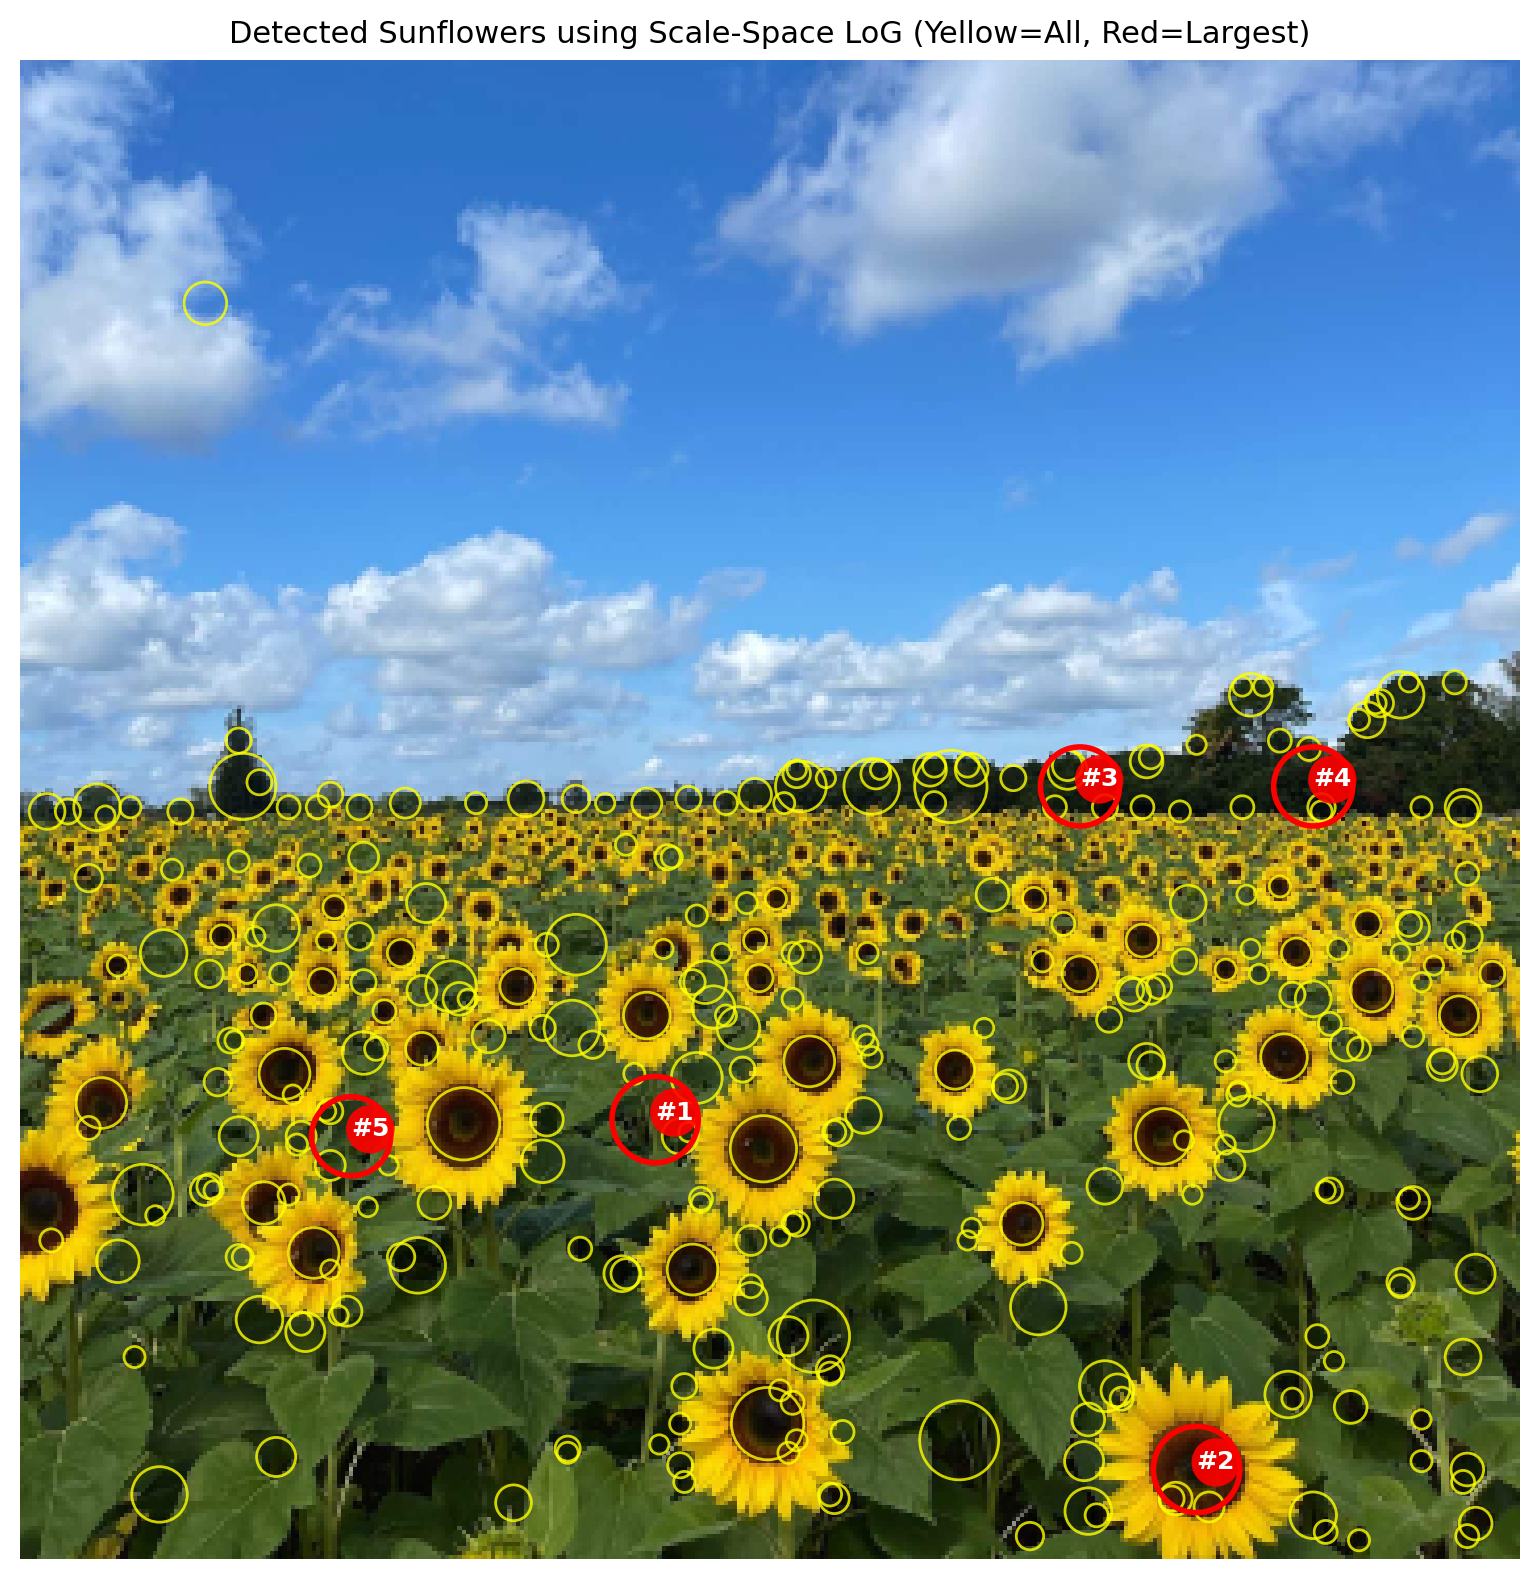
\includegraphics[width=\linewidth, keepaspectratio]{Images/task1_detected_circles.png}
			\captionof{figure}{Detected circles (yellow) with top 5 largest circles highlighted (red).}
			\label{fig:task1_detections}
		\end{minipage}
		\hfill
		\begin{minipage}[c]{0.47\textwidth}
			\centering
			\scriptsize
			\setlength{\tabcolsep}{3pt}
			\begin{tabular}{ccccc}
				\toprule
				\textbf{Rank} & \textbf{Center $(x, y)$} & \textbf{Radius $r$ (px)} & \textbf{Scale $\sigma$} & \textbf{LoG Resp.} \\
				\midrule
				1 & $(152.0, 254.0)$ & $10.36$ & $7.33$ & $0.1328$ \\
				2 & $(282.0, 338.0)$ & $10.36$ & $7.33$ & $0.3492$ \\
				3 & $(254.0, 174.0)$ & $9.49$ & $6.71$ & $0.2398$ \\
				4 & $(310.0, 174.0)$ & $9.49$ & $6.71$ & $0.1760$ \\
				5 & $(79.0, 258.0)$ & $9.49$ & $6.71$ & $0.1777$ \\
				\bottomrule
			\end{tabular}
			\captionof{table}{Parameters of the 5 largest detected circles.}
			\label{tab:largest_circles}
			\vspace{0.25cm}
			\normalsize
			\raggedright
			\footnotesize
			\textbf{Summary of Results:}
			\begin{itemize}[leftmargin=*, nosep]
				\item \textbf{Range of $\sigma$ Values Used:} $\sigma \in [1.50, 8.00]$ across 20 geometrically spaced levels ($k = 1.092$), covering radii from $2.12\text{ px}$ to $11.31\text{ px}$.
				\item \textbf{Parameters of Largest Circles:} Reported in Table \ref{tab:largest_circles}. Restricting $\sigma_{\max} = 8.00$ isolates individual flower heads (e.g., $r = 10.36\text{ px}$ at $(282.0, 338.0)$) without over-merging into background trees.
				\item \textbf{Total Detections:} A total of 314 blobs were detected across the image, successfully marking sunflower centers from the distant field to the foreground.
			\end{itemize}
		\end{minipage}
	\end{figure}

	\newpage
	\noindent\textbf{\large \color{uomaccent} 2. Line and Circle Fitting using RANSAC and Optimization}
	\vspace{0.1cm}
	
	\noindent\textbf{2.1 Methodology \& Parameter Justification} \\
	The point set $X$ ($N = 100$) consists of $50$ points conforming to a circle ($r = 10$, center $(2, 3)$, $\sigma_{\text{circ}} = 0.625$) and $50$ points conforming to a line ($y = -x + 2$, $\sigma_{\text{line}} = 1.0$).
	\begin{itemize}[leftmargin=*, nosep]
		\item \textbf{(a) RANSAC Line Fitting:} A line is characterized by unit normal $[a, b]^T$ and orthogonal distance $d$: $a x + b y - d = 0$ with constraint $\|[a, b]^T\| = 1$. A minimal sample of $s = 2$ points $p_1, p_2$ defines normal vector $\mathbf{n} = [-(y_2 - y_1), x_2 - x_1]^T / \|p_2 - p_1\|_2$ and $d = a x_1 + b y_1$. The normal error distance to the line is $e_i = |a x_i + b y_i - d|$. Because line noise has $\sigma_{\text{line}} = 1.0$, the threshold was set to $\tau_{\text{line}} = 2.0$ ($2\sigma_{\text{line}}$). Consensus minimum was set to $T_{\text{line}} = 35$ ($>70\%$ of line points). The best consensus inliers are refined via \textbf{Total Least Squares (TLS)} using SVD on centered inlier coordinates.
		\item \textbf{(b) Remnant Subtraction \& Circle Fitting:} The line consensus inliers are subtracted: $X_{\text{remnant}} = X \setminus X_{\text{line\_inliers}}$, leaving predominantly circle points. A minimal sample of $s = 3$ non-collinear points defines a circumcircle with center $(x_c, y_c)$ and radius $r$. The radial error metric is $e_i = |\|\mathbf{x}_i - (x_c, y_c)\|_2 - r|$. With circle radial noise $\sigma_{\text{circ}} = r/16 = 0.625$, the error threshold was set to $\tau_{\text{circ}} = 1.50$ ($2.4\sigma_{\text{circ}}$) with consensus minimum $T_{\text{circ}} = 30$. Using \texttt{scipy.optimize.minimize} (Nelder-Mead), the best consensus inliers are refined by minimizing $\sum_{i \in \text{inliers}} (\|\mathbf{x}_i - (x_c, y_c)\|_2 - r)^2$.
	\end{itemize}

	\vspace{0.08cm}
	\noindent\textbf{2.2 Important Code}
	\vspace{-0.15cm}
\begin{lstlisting}
import numpy as np, scipy.optimize as opt

# 1. Line RANSAC: 2-pt sample, unit normal ||[a, b]|| = 1, normal distance error < 2.0
for _ in range(1000):
    idx = np.random.choice(len(X), 2, replace=False)
    dx, dy = X[idx[1]] - X[idx[0]]
    n = np.array([-dy, dx]) / np.hypot(dx, dy)
    d = n[0] * X[idx[0], 0] + n[1] * X[idx[0], 1]
    inliers = np.where(np.abs(n[0] * X[:, 0] + n[1] * X[:, 1] - d) < 2.0)[0]
    if len(inliers) > len(best_line_inliers):
        best_line_inliers, sample_line_model, sample_line_idx = inliers, np.array([*n, d]), idx

# Refine line via Total Least Squares (TLS) SVD on consensus inliers
X_c = X[best_line_inliers] - np.mean(X[best_line_inliers], axis=0)
_, _, Vt = np.linalg.svd(X_c); tls_n = Vt[-1]
tls_d = np.dot(tls_n, np.mean(X[best_line_inliers], axis=0))

# 2. Subtract line consensus and fit circle via RANSAC on remnant
X_rem = np.delete(X, best_line_inliers, axis=0)
for _ in range(2000):
    idx = np.random.choice(len(X_rem), 3, replace=False)
    m = fit_circle_3pts(X_rem[idx[0]], X_rem[idx[1]], X_rem[idx[2]])
    if m is None or m[2] > 50: continue
    inliers = np.where(np.abs(np.hypot(X_rem[:, 0] - m[0], X_rem[:, 1] - m[1]) - m[2]) < 1.5)[0]
    if len(inliers) > len(best_circ_inliers):
        best_circ_inliers, sample_circ_model = inliers, m

# Refine circle via scipy.optimize.minimize on consensus inliers
def loss(p):
    d = np.hypot(X_rem[best_circ_inliers, 0] - p[0], X_rem[best_circ_inliers, 1] - p[1])
    return np.sum((d - p[2]) ** 2)
opt_circle = opt.minimize(loss, sample_circ_model, method='Nelder-Mead').x
\end{lstlisting}
	\vspace{-0.2cm}

	\noindent\textbf{2.3 Results \& Discussion} \\
	\vspace{-0.25cm}
	\begin{figure}[H]
		\centering
		\begin{minipage}[c]{0.47\textwidth}
			\centering
			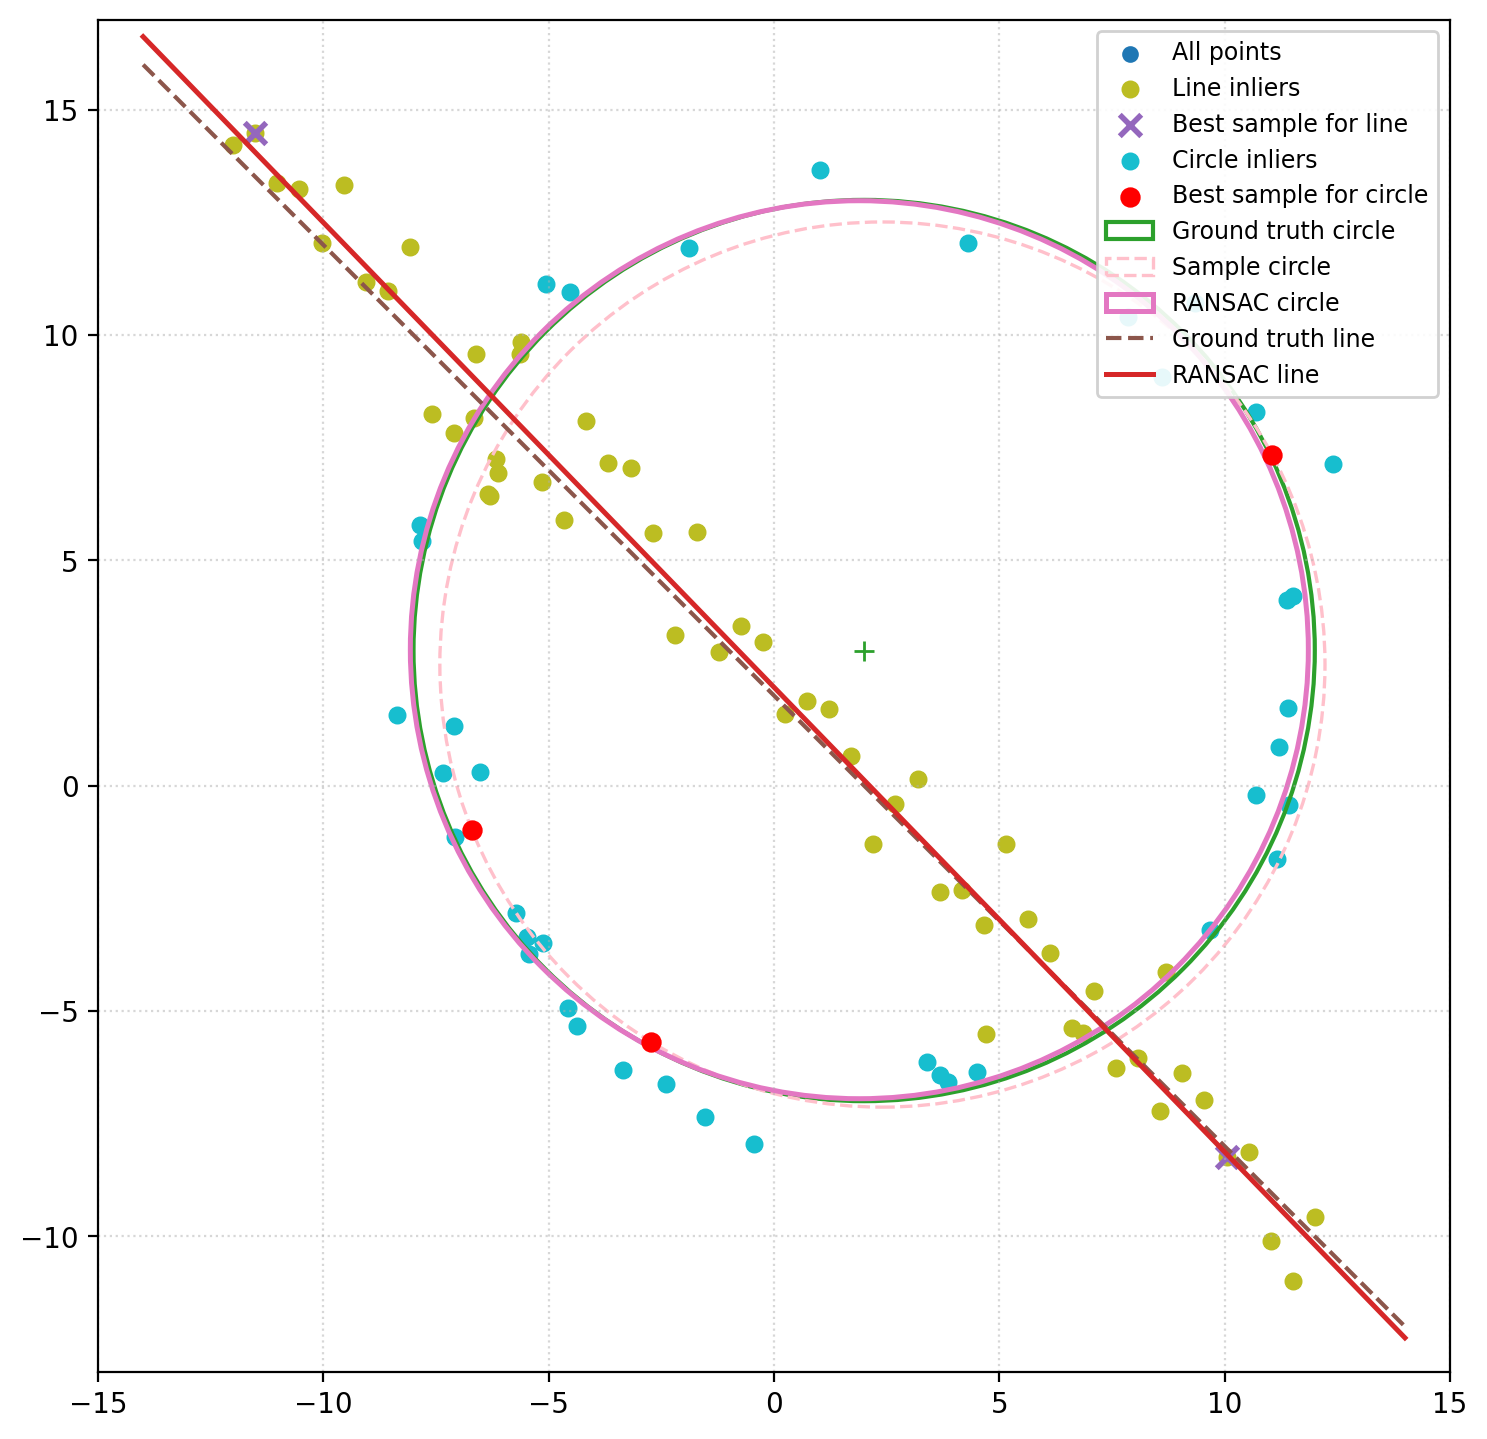
\includegraphics[height=5.6cm, keepaspectratio]{Images/task2_ransac_fitting.png}
			\captionof{figure}{Fitted line and circle with sample and inlier points.}
			\label{fig:task2_fitting}
		\end{minipage}
		\hfill
		\begin{minipage}[c]{0.51\textwidth}
			\centering
			\scriptsize
			\setlength{\tabcolsep}{2pt}
			\begin{tabular}{lcccc}
				\toprule
				\textbf{Model} & \textbf{Parameter} & \textbf{Ground Truth} & \textbf{Sample} & \textbf{Refined Fit} \\
				\midrule
				\textbf{Line} & Normal $[a, b]^T$ & $[0.71, 0.71]$ & $[-0.73, -0.69]$ & $[0.72, 0.70]$ \\
				& Distance $d$ & $1.414$ & $-1.612$ & $1.521$ \\
				& Inliers & $50$ & -- & $58$ \\
				\midrule
				\textbf{Circle} & Center $(x_c, y_c)$ & $(2.00, 3.00)$ & $(2.41, 2.69)$ & $(1.89, 3.02)$ \\
				& Radius $r$ & $10.00$ & $9.82$ & $9.96$ \\
				& Inliers & $50$ & -- & $42$ \\
				\bottomrule
			\end{tabular}
			\captionof{table}{Model parameter estimation comparison.}
			\label{tab:task2_models}
			\vspace{0.15cm}
			\normalsize
			\raggedright
			\footnotesize
			\textbf{(d) What happens if we fit the circle first?}
			\begin{itemize}[leftmargin=*, nosep]
				\item \textbf{Secant Line Contamination:} The line cuts through the circle. Fitting the circle first causes line points along the intersection to fall within radial error $\tau_{\text{circ}} = 1.50$, falsely claiming $11$ line points ($61$ total inliers).
				\item \textbf{Remnant Truncation:} Removing the corrupted circle consensus punches a hole through the line, fracturing it and biasing subsequent line estimation.
				\item \textbf{Line-First Robustness:} A line can intersect a circle at at most $2$ points. Thus, the line cannot over-fit the circle, leaving the circular remnant intact.
			\end{itemize}
		\end{minipage}
	\end{figure}

	\newpage
	\noindent\textbf{\large \color{uomaccent} 3. Planar Homography and Image Warping}
	\vspace{0.1cm}
	
	\noindent\textbf{3.1 Methodology \& Planar Homography Derivation} \\
	A planar homography is a projective transformation $\mathbf{x}' \sim \mathbf{H}\mathbf{x}$ mapping points from one planar projective plane $\mathbf{x} = [x, y, 1]^T$ to another $\mathbf{x}' = [x', y', 1]^T$ via a non-singular $3 \times 3$ matrix $\mathbf{H}$ with $8$ degrees of freedom (scale invariant). Each point correspondence $(x_i, y_i) \leftrightarrow (x'_i, y'_i)$ gives two independent linear equations:
	\begin{equation*}
		x'_i = \frac{h_{11}x_i + h_{12}y_i + h_{13}}{h_{31}x_i + h_{32}y_i + h_{33}}, \qquad y'_i = \frac{h_{21}x_i + h_{22}y_i + h_{23}}{h_{31}x_i + h_{32}y_i + h_{33}}
	\end{equation*}
	Selecting $4$ coplanar point correspondences uniquely determines $\mathbf{H}$ via Direct Linear Transformation (DLT) using \texttt{cv2.getPerspectiveTransform}. The overlay is warped into the target perspective using inverse backward mapping (\texttt{cv2.warpPerspective}) with bilinear interpolation. To faithfully replicate Figure 2 of the assignment, the warped flag is blended onto the target wall polygon via additive blending: $\mathbf{I}_{\text{blend}} = \mathbf{I}_{\text{target}} + 0.5\,\mathbf{I}_{\text{warped}}$. For overlays with transparent backgrounds, alpha-compositing is applied.

	\vspace{0.08cm}
	\noindent\textbf{3.2 Important Code}
	\vspace{-0.15cm}
\begin{lstlisting}
import cv2, numpy as np

def superimpose_image(target_path, overlay_path, dst_pts, mode='additive', alpha=0.5):
    target = cv2.imread(target_path)
    overlay = cv2.imread(overlay_path, cv2.IMREAD_UNCHANGED)
    h_ov, w_ov = overlay.shape[:2]
    src_pts = np.float32([[0, 0], [w_ov - 1, 0], [w_ov - 1, h_ov - 1], [0, h_ov - 1]])
    
    # 1. Planar homography matrix H mapping overlay corners -> target planar coordinates
    H = cv2.getPerspectiveTransform(src_pts, dst_pts.astype(np.float32))
    warped = cv2.warpPerspective(overlay, H, (target.shape[1], target.shape[0]))
    
    # 2. Construct polygon mask for planar region
    mask = np.zeros(target.shape[:2], dtype=np.uint8)
    cv2.fillConvexPoly(mask, dst_pts.astype(np.int32), 255)
    
    # 3. Blend warped overlay onto target architectural surface
    res = target.copy()
    if mode == 'additive':  # Replicates Figure 2: target + 0.5 * warped
        res[mask > 0] = cv2.add(res[mask > 0], (warped[mask > 0, :3] * alpha).astype(np.uint8))
    elif mode == 'alpha':     # Alpha transparency compositing
        a = (warped[:, :, 3].astype(float) / 255.0)[:, :, None]
        res = np.clip(res.astype(float) * (1 - alpha * a) + warped[:, :, :3] * (alpha * a), 0, 255).astype(np.uint8)
    return res, H
\end{lstlisting}
	\vspace{-0.15cm}

	\noindent\textbf{3.3 Results, Observations \& Non-Technical Rationale}
	\vspace{-0.2cm}
	\begin{figure}[H]
		\centering
		\begin{subfigure}[b]{0.485\textwidth}
			\centering
			\includegraphics[height=3.6cm, keepaspectratio]{Images/task3_wadham_pts.png}
			\caption{Pair 1: Wadham College 4 clicked corners}
		\end{subfigure}
		\hfill
		\begin{subfigure}[b]{0.485\textwidth}
			\centering
			\includegraphics[height=3.6cm, keepaspectratio]{Images/task3_wadham_superimposed.png}
			\caption{Pair 1: Superimposed British flag (Fig. 2 replication)}
		\end{subfigure}
		
		
		\caption{Planar homography superimposition on architectural surfaces.}
		\label{fig:task3_superimposition}
	\end{figure}
	\vspace{-0.35cm}

	\noindent\begin{minipage}[t]{0.48\textwidth}
		\footnotesize \textbf{Pair 1: Wadham College \& UK Flag (Figure 2 Replication)}
		\begin{itemize}[leftmargin=*, nosep]
			\item \textbf{Selected 4 Points:} $P_1(147, 208)$, $P_2(517, 292)$, $P_3(521, 521)$, $P_4(135, 519)$ on the receding quadrangle facade.
			\item \textbf{Non-Technical Rationale:} Contextual alignment of Oxford University's historic 17th-century Wadham College with the British Union Jack, celebrating British collegiate heritage.
			\item \textbf{Observation:} Additive blending preserves underlying window mullions and stone masonry textures, replicating a semi-transparent projection.
		\end{itemize}
	\end{minipage}
	\hfill
	\begin{minipage}[t]{0.48\textwidth}
		\footnotesize \textbf{Pair 2: Engineering Facade \& UoM Coat of Arms}
		\begin{itemize}[leftmargin=*, nosep]
			\item \textbf{Selected 4 Points:} $P_1(382, 346)$, $P_2(454, 262)$, $P_3(454, 552)$, $P_4(382, 602)$ along vertical concrete bay columns.
			\item \textbf{Non-Technical Rationale:} Modern institutional branding, virtually mounting the official University of Moratuwa crest on the structural concrete facade of the School of Engineering.
			\item \textbf{Observation:} Preserves geometric foreshortening as the building recedes towards the vanishing point, appearing as an authentic architectural installation.
		\end{itemize}
	\end{minipage}

\end{document}